%\documentclass{nitocs}
\documentclass[summary]{nitocs}
% \documentclass[summary,draft]{nitocs} % 画像がコンパイルされない


\usepackage[dvipdfmx]{graphicx}
\usepackage{latexsym}
\usepackage{bm}
\usepackage{amsmath}
\numberwithin{equation}{section}
\graphicspath{{./IMG/}} % 画像指定用のパス

\renewcommand{\theequation}{\arabic{equation}}
\renewcommand{\thefigure}{\arabic{section}.\arabic{figure}}
\renewcommand{\thetable}{\arabic{section}.\arabic{subsection}.\arabic{table}}
\makeatletter
\@addtoreset{equation}{section}
\@addtoreset{figure}{section}
\@addtoreset{table}{section}
\setlength{\mathindent}{0pt}
% 
\def\Underline{\setbox0\hbox\bgroup\let\\\endUnderline}
\def\endUnderline{\vphantom{y}\egroup\smash{\underline{\box0}}\\}
\def\|{\verb|}

\setcounter{page}{1}
\begin{document}

    \title{囲碁における盤面識別システムの検討}
    \author{橋本 燎}{Ryo Hashimoto} % 氏名
    \advisor{井上 優良}{Yusuke Inoue}   % 指導教員氏名

    % 実行時の日付が自動挿入されるはず
    \date{令和3年\number\month 月\number\day 日} 

    \maketitle
    \section{緒言} \label{intro}
            % 囲碁について
        囲碁は,2人のプレイヤーが碁石を碁盤へ配置するボードゲームである.碁石は各プレイヤーが使用する白黒の石であり,碁盤は通常$19\times19$の格子状の盤面のことを指す.
        このゲームは両プレイヤーが碁石を交互に碁盤上に設置し,碁石で囲まれた陣地を多く確保したプレイヤーが勝利する.
        相手の陣地として成立している領域でなければどこにでも碁石を置くことができる,相手プレイヤーの碁石を陣地内に収めることでその碁石を奪い使用することで相手陣地の縮小を行うことができる等,
        ルール上の制約が極めて少ないといった特徴を持つため,他のボードゲームと比較すると可能な総局面数は膨大になる.

        近年,様々な人工知能が登場しプロ棋士との対局が行われてきたが,これらの対局の様子を見ると,プロ棋士の置いた石の配置をコンピュータに入力する役割を持った人間が存在していた.
        そこで,人の手による記録作業を行わずに対局の状況を記録できるシステムの構築を目指す.

            % 研究について
        本研究では,対局中の囲碁の画像から碁石の配置を識別するシステムの検討を行う.
        その後,複数の画像に対してシステムを試し,結果を考察する.

    \section{理論} \label{theory}
        \subsection{同次座標}
            座標$(x,y)$に対し,その要素を1つ増やした座標$(\xi_1,\xi_2,\xi_3)$を,以下の関係式を満たすように定義する.\\
            \begin{equation} % 同次座標の数式
                    x = \frac{\xi_1}{\xi_3}, \;\;\;\;\;\;\;\; y = \frac{\xi_2}{\xi_3}
                \label{Homogeneous}
            \end{equation}

            ただし,$\xi_1,\xi_2,\xi_3$のうち少なくとも1つは0ではないとする.このように定義される座標を同次座標と呼ぶ\cite{DIP}.

            同次座標においては$\lambda\neq0$なる任意の$\lambda$に対して,$(\xi_1,\xi_2,\xi_3)$と$(\lambda\xi_1,\lambda\xi_2,\lambda\xi_3)$は通常の座標に直したときともに$(\xi_1/\xi_3,\xi_2/\xi_3)$となるため,同じ点を表している.つまり,同次座標による表現では,定数倍をしても変わらないとみなすことができる.このような表現を同値であるとよび,これを式では以下のように表す.
            \begin{equation} % 同次座標の数式2
                \left(
                    \begin{array}{ccc}
                        \xi_1\\
                        \xi_2\\
                        \xi_3
                    \end{array}
                \right) \sim % \sim: 「~」
                \left(
                    \begin{array}{ccc}
                        \lambda\xi_1\\
                        \lambda\xi_2\\
                        \lambda\xi_3
                    \end{array}
                \right)
            \end{equation}
            ここで記号$\sim$は同値関係を表し,定数倍の違いを許して等しいことを意味する.

        \subsection{射影変換}
            同次座標を利用することにより,一般的な変換を表現することができる.
            これは以下の式で表現されるもので,射影変換と呼ばれている\cite{DIP}.
            \begin{equation} % 射影変換の数式
                \left(
                    \begin{array}{ccc}
                    x'\\
                    y'\\
                    1
                    \end{array}
                \right)\sim
                \left(
                    \begin{array}{ccc}
                    h_{11} & h_{12} & h_{13}\\
                    h_{21} & h_{22} & h_{23}\\
                    h_{31} & h_{32} & h_{33}\\
                    \end{array}
                \right)
                \left(
                    \begin{array}{ccc}
                    x\\
                    y\\
                    1
                    \end{array}
                \right)
                \label{Homography}
            \end{equation}

            射影変換においては,線分の直線性は保たれるものの,平行性は失われる.別の言い方をすると,任意の四角形を別の任意の四角形に移すような変換であるといえる.
                %! 模式図を入れる余裕がないかもしれない
            %     %? 「概略図」? なんかパッとしない表現 -> 「模式図」にしてみた
            % 射影変換の模式図を図\ref{sample_homography}に示す.
            % \begin{figure}[tb] % 射影変換の模式図
            %     \begin{center}
            %     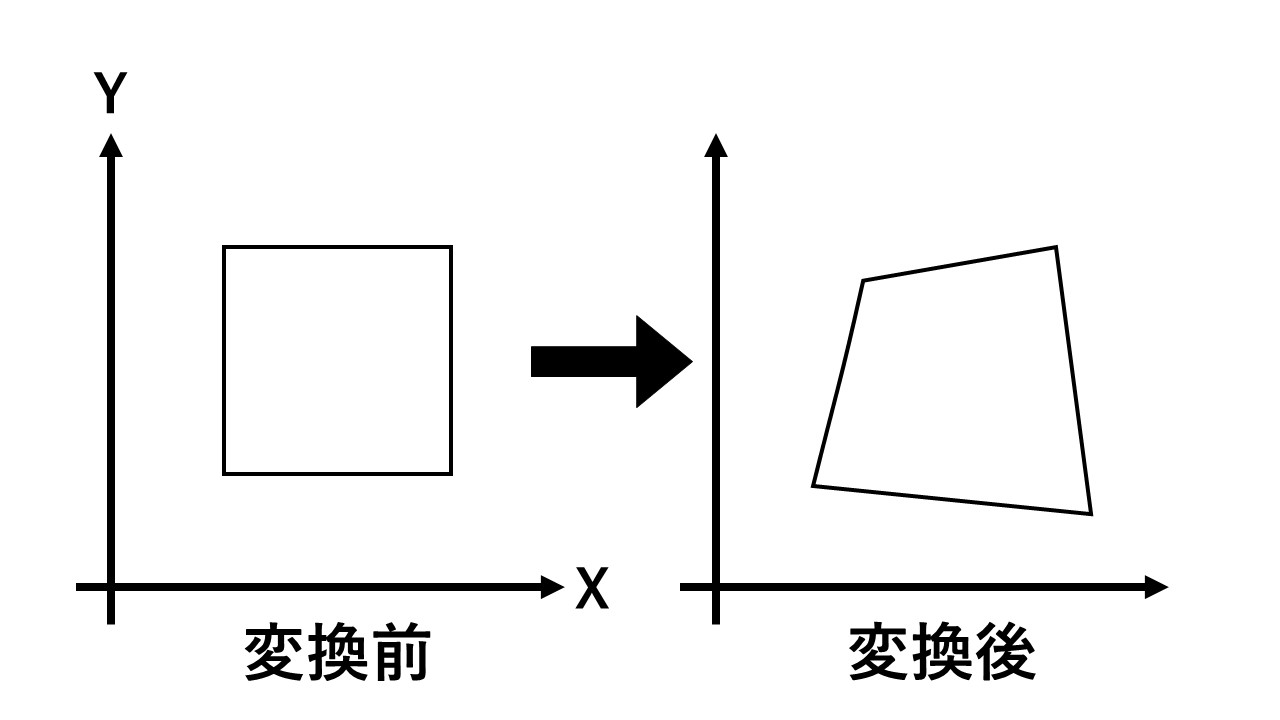
\includegraphics[clip,width=80mm]{Homography.jpg} 
            %     \caption{射影変換の模式図}
            %     \label{sample_homography}
            %     \end{center}
            % \end{figure}

        \subsection{メディアンフィルタ}
            フィルタ範囲内のピクセルの画素値を昇順か降順に並び替え,中央値を出力するフィルタをメディアンフィルタと呼ぶ\cite{DIP}.
            このフィルタは,コントラストの差がある輪郭部分がぼやけにくい特徴を持つ.


    \section{盤面識別システム} \label{system}
        システムは,与えられた画像に対して以下の前処理を行う.
        \begin{itemize}
            \item 射影変換(盤面部分の切り抜き)
            \item グレースケール化
            \item ノイズ除去(格子線の除去)
        \end{itemize}
        前処理が完了した画像に対して,システムは$19\times19$個の小さな領域を付与する.
        この領域内に存在する画素値の平均と,設定したしきい値をもとに,システムは各領域の位置に置かれている石の種類の識別を行う.

        前処理におけるノイズ除去にはメディアンフィルタを使用する.
        なぜならば,メディアンフィルタは輪郭部分を残しやすいという特徴を持っているためである.
        たとえば平均値フィルタ(範囲内の画素値の平均を出力するフィルタ)は輪郭も曖昧にしてしまうという特徴がある.
        これに対し,メディアンフィルタは輪郭を残しやすいため,碁石の色が滲むことを防ぐことができる.
        碁石のある碁盤に,平均値フィルタとメディアンフィルタを適用した例をそれぞれ図\ref{average},図\ref{median}に示す.
        \begin{figure}[tb] % 事例2,誤り部分・領域可視化版の2枚セット
            \begin{center}
              \begin{tabular}{c}
                \begin{minipage}{0.5\hsize}
                  \begin{center}
                    \includegraphics[clip,width=30mm]{blur_result.jpg}
                \caption{平均値フィルタ}
                \label{average}
                  \end{center}
                \end{minipage}
                \begin{minipage}{0.5\hsize}
                  \begin{center}
                    \includegraphics[clip,width=30mm]{median_result.jpg}
                \caption{メディアンフィルタ}
                \label{median}
                  \end{center}
                \end{minipage}
              \end{tabular}
            \end{center}
        \end{figure}


        % 理由は? 
            %TODO 必要であれば領域付与済みの図を入れる

    \section{実験} \label{experiment}
        システムの有効性を検証するため,実際に盤面を含む画像を使ってシステムを適用し結果を考察する.
        %? 輝度値の決定方法について述べる余裕があるか?
        \subsection{石の位置ずれ} \label{ex2}% 位置ズレによる失敗.DSC_0099.
            この盤面画像(図\ref{ex2_img})に対してシステムを適用した.
            実際の配置と比較して,システムが「石がない」と誤った部分にマークを付け,その周囲を拡大したものを図\ref{ex2_error}に示す.

            図\ref{ex2_error}の範囲にグレースケール化とノイズ除去を適用し,輝度値の平均を取得する領域を緑色の四角形で表した画像を図\ref{ex2_error_area}に示す.
            図\ref{ex2_error_area}を見ると,中央の白石の大部分が領域からはみ出ているのが分かる.
            このことから,石が正しく盤面の交点上に配置されていない場合,システムは正常に石を識別できないと考える.
            
            \begin{figure}[tb] % 事例2_盤面
                \begin{center}
                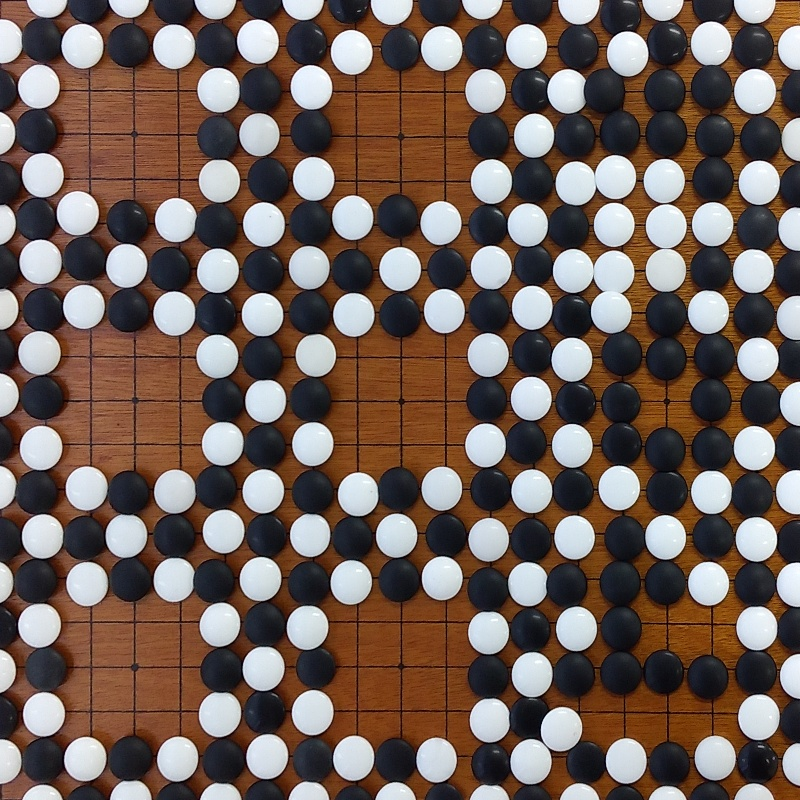
\includegraphics[clip,width=50mm]{DSC_0099/boardImg.jpg} 
                \caption{\ref{ex2}節で使用した盤面画像}
                \label{ex2_img}
                \end{center}
            \end{figure}

            %! 指摘された,誤り箇所を2枚並べにする修正
                %TODO これを論文の再提出版にも行え.
            \begin{figure}[tb] % 事例2,誤り部分・領域可視化版の2枚セット
                \begin{center}
                  \begin{tabular}{c}
                    \begin{minipage}{0.5\hsize}
                      \begin{center}
                        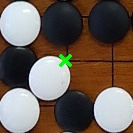
\includegraphics[clip,width=30mm]{DSC_0099/TRIM_resultCompare.jpg}
                    \caption{図\ref{ex2_img}の誤り部分}
                    \label{ex2_error}
                      \end{center}
                    \end{minipage}
                    \begin{minipage}{0.5\hsize}
                      \begin{center}
                        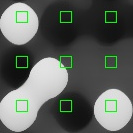
\includegraphics[clip,width=30mm]{DSC_0099/TRIM_boardWithAreaImg.jpg}
                    \caption{誤り部分の領域を可視化}
                    \label{ex2_error_area}
                      \end{center}
                    \end{minipage}
                  \end{tabular}
                \end{center}
            \end{figure}


        \subsection{碁盤の反射光} \label{reflection}% 反射による失敗.DSC_0098.
            この盤面画像(図\ref{ex3_img})に対してシステムを適用した.
            実際の配置と比較して,システムが白石と誤った部分にマークを付け,その周囲を拡大したものを図\ref{ex3_error}に示す.

            図\ref{ex3_error}の範囲に対し,白石の識別に用いるしきい値よりも暗い部分を黒,明るい部分を白とした二値画像を図\ref{ex3_error_area}に示す.
            図\ref{ex3_error_area}を見ると,白石が無い部分もしきい値より明るいことが分かる.
            このことから,盤面や黒石に反射光が含まれていると,システムは誤って白石と識別してしまうと考える.
            \begin{figure}[tb] % 事例3_盤面
                \begin{center}
                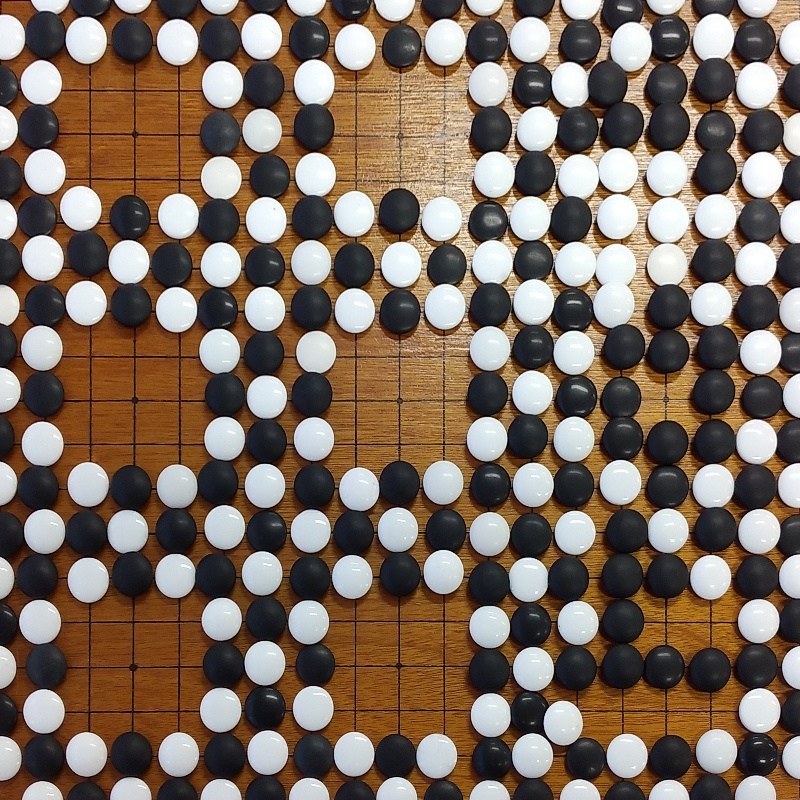
\includegraphics[clip,width=50mm]{DSC_0098/boardImg.jpg} 
                \caption{\ref{reflection}節で使用した盤面画像}
                \label{ex3_img}
                \end{center}
            \end{figure}

            \begin{figure}[tb] % 事例3,誤り部分,二値画像の2枚セット
                \begin{center}
                  \begin{tabular}{c}
                    \begin{minipage}{0.5\hsize}
                      \begin{center}
                        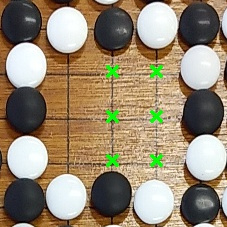
\includegraphics[clip,width=30mm]{DSC_0098/TRIM_resultCompare.jpg}
                    \caption{図\ref{ex3_img}の誤り部分}
                    \label{ex3_error}
                      \end{center}
                    \end{minipage}
                    \begin{minipage}{0.5\hsize}
                      \begin{center}
                        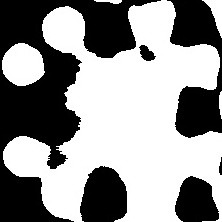
\includegraphics[clip,width=30mm]{DSC_0098/TRIM_inRange_WHITE.jpg}
                    \caption{誤り部分の二値化}
                    \label{ex3_error_area}
                      \end{center}
                    \end{minipage}
                  \end{tabular}
                \end{center}
            \end{figure}




    \section{結言}\label{conclusion} % 結言
        本研究で検討したシステムでは,石の位置に大きなずれが無い,かつ反射光が写り込んでいない場合に限り,碁石を正常に識別することができた.
        石のずれに対応できない問題には,碁石の位置を碁盤の交点や石の形状をもとに検出することで問題を解決できると考える.
        反射光を白石と識別していまう問題には,しきい値を固定するのではなく画像に応じて適切なしきい値を算出することや,画像上の反射光の写り込みを軽減させるノイズ処理を適用することで,誤った識別をする数を減らすことができると考える.
        よって,今後の課題として
        \begin{itemize}
            \item 石の座標を検出する手法
            \item 画像の状況に応じて適切なしきい値を算出する手法
            \item 反射光を軽減させる画像処理の手法
        \end{itemize}
        の模索が挙げられる.    

    \begin{thebibliography}{10}
        %! 参考文献
        % 著者名,書名,編者名,発行所,発行都市名,発行年.

        \bibitem{DIP}
        江尻 正員ほか,
        ディジタル画像処理[改訂第二版],
        奥富 正敏,
        CG-ARTS,
        2020.
    \end{thebibliography}

\end{document}
